
%(BEGIN_QUESTION)
% Copyright 2011, Tony R. Kuphaldt, released under the Creative Commons Attribution License (v 1.0)
% This means you may do almost anything with this work of mine, so long as you give me proper credit

Undersøk denne closed-loop-trenden fra en væskeflow-reguleringsprosess:

$$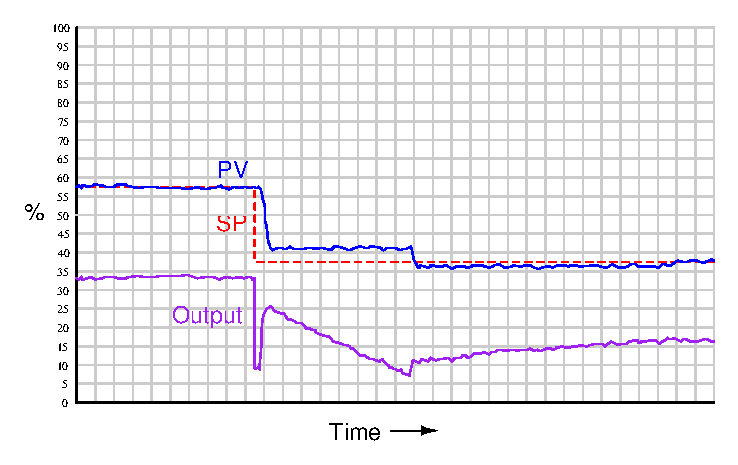
\includegraphics[width=15.5cm]{i00288x01.eps}$$

Identifiser om dette er en \textit{P-only}, \textit{I-only}, \textit{P+I}, \textit{P+D}, eller full \textit{PID}-kontroller, basert på trendene.

\vskip 10pt

Identifiser også om kontrolleren er \textit{direct-acting} eller \textit{reverse-acting}.

\vskip 10pt

Identifiser til slutt problemet i sløyfen, og forklar hvordan trendene viser dette.

\vskip 50pt

\underbar{file i00288}
%(END_QUESTION)





%(BEGIN_ANSWER)

{\bf 2 poeng:} Dette er en {\bf P+I}-kontroller (ingen derivasjonsledd).

\vskip 10pt

{\bf 2 poeng:} Kontrolleren er konfigurert for {\bf reverse} virkning.

\vskip 10pt

{\bf 2 poeng:} Problemet er en treg/sticky reguleringsventil.

\vskip 10pt

{\bf 4 poeng:} Vi identifiserer dette på hvor lenge PV blir liggende unna SP til tross for at integralleddet fortsetter å vikle ned.

%(END_ANSWER)





%(BEGIN_NOTES)

{\bf This question is intended for exams only and not worksheets!}.

%(END_NOTES)
